\documentclass[landscape,a0paper,fontscale=0.292]{baposter}

\usepackage{macros}

 
%%%%%%%%%%%%%%%%%%%%%%%%%%%%%%%%%%%%%%%%%%%%%%%%%%%%%%%%%%%%%%%%%%%%%%%%%%%%%
%% Begin of Document
%%%%%%%%%%%%%%%%%%%%%%%%%%%%%%%%%%%%%%%%%%%%%%%%%%%%%%%%%%%%%%%%%%%%%%%%%%%%%
\begin{document}
%%%%%%%%%%%%%%%%%%%%%%%%%%%%%%%%%%%%%%%%%%%%%%%%%%%%%%%%%%%%%%%%%%%%%%%%%%%%%
%% Here starts the poster
%%---------------------------------------------------------------------------
%% Format it to your taste with the options
%%%%%%%%%%%%%%%%%%%%%%%%%%%%%%%%%%%%%%%%%%%%%%%%%%%%%%%%%%%%%%%%%%%%%%%%%%%%%
\begin{poster}
{
 % Show grid to help with alignment
 grid=false,
 % Column spacing
 colspacing=1.4em,
 % Color style
 headerColorOne=vividcerise!30!white!90!black,
 borderColor=vividcerise!35!white!90!black,
 % Format of textbox
 textborder=faded,
 % Format of text header
 headerborder=open,
 headershape=roundedright,
 headershade=plain,
 background=none,
 %bgColorOne=vividcerise!10!white,
 headerheight=0.12\textheight}
 % Eye Catcher
 {
 }
 % Title
 {\sc\LARGE \bf{(Bandit) Convex Optimization with Biased Noisy Gradient Oracles} \vspace{1ex}}
 % Authors and affiliations
 {Xiaowei  Hu \hspace{1em} Prashanth L A \hspace{1em} Andr\'as Gy\"orgy \hspace{1em} Csaba Szepesv\'ari}
 % University logo
 {
\begin{tabular}{ccc}

\includegraphics[width=3cm,height=1.4cm]{fig/u-of-alberta-logo}& 

\includegraphics[width=3cm,height=1.7cm]{fig/clark.png} &

\includegraphics[width=3cm,height=1.5cm]{fig/icl.png} 
\end{tabular}
}

%%%%%%%%%%%%%%%%%%%%%%%%%%%%%%%%%%%%%%%%%%%%%%%%%%%%%%%%%%%%%%%%%%%%%%%%%%%%%%
%%% Now define the boxes that make up the poster
%%%%%%%%%%%%%%%%%%%%%%%%%%%%%%%%%%%%%%%%%%%%%%%%%%%%%%%%%%%%%%%%%%%%%%%%%%%%%%
\headerbox{Convex Opt + Noisy Feedback}{name=setting,column=0,row=0,span=2}{
\begin{tabular}[b]{cc}
\begin{minipage}{0.37\textwidth}
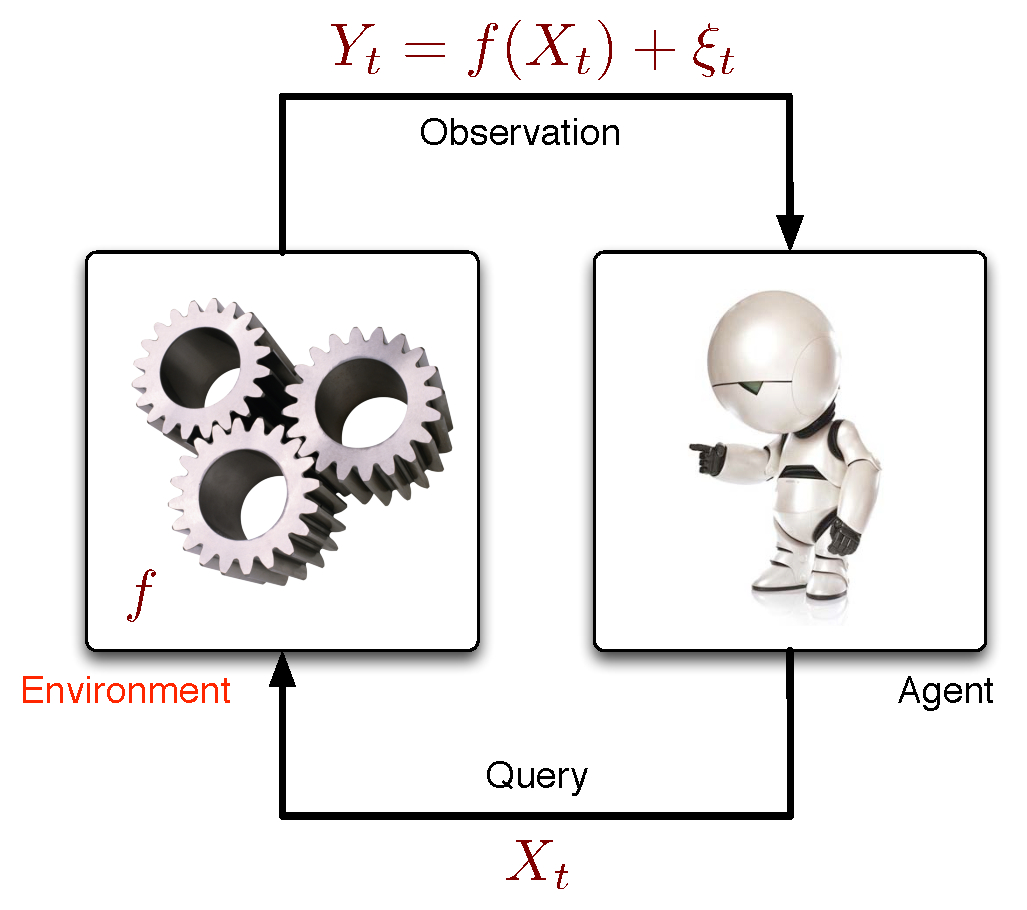
\includegraphics[scale=0.32]{fig/Interaction} 
\end{minipage} &
\begin{minipage}{0.61\textwidth}
\textbf{Assume $f$ convex + smooth}\\[1.5ex]
\textbf{{\color{red!80!black} Goal:} Find a near-minimizer of $f$ using $n>0$ queries!
}\\[2.5ex]
\tikz[baseline]{
            \node[trapezium,trapezium left angle=100,
  trapezium right angle=100, fill=red!20,anchor=base] (t1)
            {\makecell{\large \textbf{How fast can the optimization error}\\[1.5ex]
		$\bm{\Delta_n = \EE{f(X_n) }- \inf_{x\in \cK} f(x)}$\\[1.5ex]
		 \large \textbf{decrease with $n$?}
}};}	


\end{minipage} 
\end{tabular}

}


\headerbox{Biased Gradient Oracle}{name=oracle,column=0,below=setting,span=2}{
\begin{center}
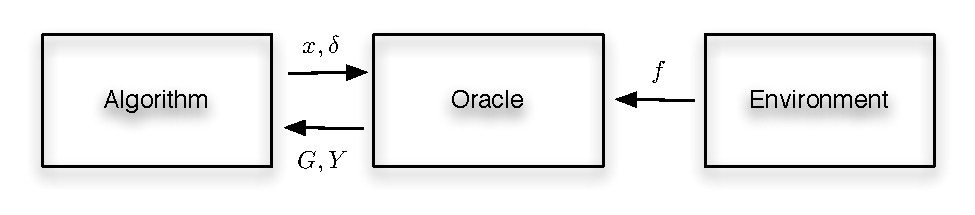
\includegraphics[scale=0.7]{fig/oracle0}	
\end{center}

\begin{large}
\begin{tabular}{cccc}
\tikz[baseline]{
            \node[ellipse,minimum width=50pt, minimum height=20pt, fill=blue!20,anchor=base] (t1)
            {\textbf{Bias}};} 
& 
\tikz[baseline]{
            \node[rectangle,minimum height=20pt, fill=magenta!30,anchor=base] (t1)
            {$\bm{\norm{ \EE{G}  - \nabla f(x)  }_* \le c_1(\delta)}$};} 
  
&
\tikz[baseline]{
            \node[ellipse, minimum width=70pt, minimum height=20pt,fill=blue!20,anchor=base] (t1)
            {\textbf{Second moment}};} 
&
\tikz[baseline]{
            \node[rectangle,minimum height=20pt, fill=yellow!30,anchor=base] (t1)
            {$\bm{\EE{\norm{ G  }_*^2} \le c_2(\delta)}$};} \\[2ex]
\end{tabular}

\begin{center}
\tikz[baseline]{
            \node[trapezium,trapezium left angle=70,
  trapezium right angle=-70, fill=asparagus!60, minimum height=10pt,text=black,anchor=base] (t1)
            {\textbf{Polynomial oracle:} $\bm{c_1(\delta) = C_1 \delta^p, c_2(\delta) = C_2 \delta^{-q}, p,q>0}$};}	
\end{center}



\end{large}

}

%%%%%%%%%%%%%%%%%%%%%%%%%%%%%%%%%
\headerbox{Sample Oracles}{name=sampleoracles,column=0,below=oracle,span=2}{
\begin{tabular}{cc}
\tikzstyle{mybox} = [draw=blue, fill=green!20, very thick,
    rectangle, rounded corners, inner sep=20pt, inner ysep=20pt]
\tikzstyle{fancytitle} =[fill=blue, text=white, ellipse,minimum height=20pt]
%
\begin{tikzpicture}[transform shape, baseline=-3.5cm]
\node [mybox] (box) {%
    \begin{minipage}[t!]{.43\textwidth}
$\bm{G = \frac{ (f(x+U)+\xi^+) - (f(x-U)+\xi^-)}{2} V\,}$
    \end{minipage}
    };
\node[fancytitle] at (box.north) {Two-point estimate};
\end{tikzpicture}


& 
%%%%
\tikzstyle{mybox} = [draw=blue, fill=blue!20, very thick,
    rectangle, rounded corners, inner sep=20pt, inner ysep=20pt]
\tikzstyle{fancytitle} =[fill=blue, text=white, ellipse,minimum height=20pt]
%
\begin{tikzpicture}[transform shape, baseline=-3.5cm]
\node [mybox] (box2) {%
    \begin{minipage}[t!]{.3\textwidth}
$\bm{G =  (f(x+U)+\xi)  V\,}$
    \end{minipage}
    };
\node[fancytitle] at (box2.north) {One-point estimate};
\end{tikzpicture}
\end{tabular}

\vspace{-15ex}

\begin{center}
	\tikz[baseline]{
            \node[fill=red!20,anchor=base] (t1)
            {\textbf{\large Choose $\bm{U,V}$ such that $\bm{\EE{ V U^\top  } = I}$, $\bm{\EE{ V } = 0}$.} };
            }
\end{center}

\begin{center}
	\tikz[baseline]{
            \node[fill=red!20,anchor=base] (t1)
            {A popular choice: $U=\delta u$, $V=\dfrac{d}{\delta}u$, $u$ is random unit vector};
            }
\end{center}

%\begin{tikzpicture}[overlay]
%        \path[thick,->] (box) edge [bend right] (t1);
%        \path[thick,->] (box2) edge [bend left] (t1);
%\end{tikzpicture}

Covers  {\color{blue!80} Katkovnik and Kulchitsky (1972), Polyak and Tsybakov (1990), Dippon (2003); Nesterov (2011), Kushner and Clark (1978), Flaxman et al. (2005), Spall (1992), $\ldots$}

\begin{center}
\tikz[baseline]{
            \node[trapezium,trapezium left angle=100,
  trapezium right angle=100, fill=antiquefuchsia!90,text=black,anchor=base] (t1)
            {\makecell{\large \textbf{	Does it matter which of these we select? Not really:}\\[1.5ex]
		\large \textbf{Bias: $\bm{O(\delta^2)}$, second moment: $\bm{O(1)}$ or $\bm{O(\delta^{-2})}$}}};}	
\end{center}

}

%%%%%%%%%%%%%%%%%%%%%%%%%%%%%%%%%
\headerbox{Lower Bound}{name=lowerbound,column=2,row=0,span=2, headerColorOne=teagreen, borderColor=teagreen}{
\textbf{\color{upmaroon} Notation:} 
\tikz[baseline]{
            \node[ellipse, minimum width=50pt, minimum height=20pt,fill=blue!20,anchor=base] (t1)
            {$\bm{\F_{L,0}}$};}  $\rightarrow$ \textbf{\color{tealgreen} Convex + $L$-smooth} \hspace{2em} 
						\tikz[baseline]{
            \node[ellipse, minimum width=50pt, minimum height=20pt,fill=green!20,anchor=base] (t1)
            {$\bm{\F_{L,1}}$};}
						$\rightarrow$ \textbf{\color{tealgreen} $1$-Strongly Convex + $L$-smooth}\\[1.5ex] 

%%%%
\tikzstyle{mybox} = [draw=blue, fill=antiquefuchsia!40, very thick,
    rectangle, rounded corners, inner sep=20pt, inner ysep=20pt]
\tikzstyle{fancytitle} =[fill=red!30, text=black, ellipse,minimum height=20pt]
\begin{large}
\begin{tikzpicture}[transform shape, baseline=-3.5cm]
\node [mybox] (box2) {%
    \begin{minipage}[t!]{.91\textwidth}
$\cK\subset \R^d$ convex, closed, with  $\{+1,-1\}^d\subset \cK$, $n$ large enough.\\[1.5ex]
For any algorithm $\mathrm{A}$ that observes $n$ random elements from a  $(p,q)$ polynomial oracle, we have

\begin{tabular}{cc}
\hspace{-2em}						\tikz[baseline]{
            \node[draw=black,minimum width=20pt,fill=teagreen,anchor=base] (t1)
            {$\bm{\Delta_n(\F_{L,0},\mathrm{A},c_1,c_2 )} \bm{= \Omega( n^{-\frac{p}{2p+q}})}$};}
&
						\tikz[baseline]{
            \node[draw=black,minimum width=20pt,fill=shockingpink!20,anchor=base] (t1)
            {$\bm{\Delta_n(\F_{L,1},\mathrm{A},c_1,c_2 )} \bm{ = \Omega(  n^{-\frac{2p}{2p+q}})}$};}
\end{tabular}
    \end{minipage}
    };
\node[fancytitle] at (box2.north) {\textbf{\Large Main Result}};
\end{tikzpicture}
\end{large}
}

%%%%%%%%%%%%%%%%%%%%%%%%%%%%%%%%%
\headerbox{Upper Bound}{name=upperbound,column=2,below=lowerbound,span=2, headerColorOne=teagreen, borderColor=teagreen}{
\textbf{\color{upmaroon} Algorithm:} 
\tikz[baseline]{
            \node[ellipse, minimum width=80pt, minimum height=20pt,fill=blue!20,anchor=base] (t1)
            {\textbf{Mirror Descent (MD)}};} \\[1.5ex] 

%%%%
\tikzstyle{mybox} = [draw=blue, fill=sandybrown!40, very thick,
    rectangle, rounded corners, inner sep=20pt, inner ysep=20pt]
\tikzstyle{fancytitle} =[fill=blue!30, text=black, ellipse,minimum height=20pt]
\begin{large}
\begin{tikzpicture}[transform shape, baseline=-3.5cm]
\node [mybox] (box2) {%
    \begin{minipage}[t!]{.91\textwidth}

\begin{tabular}{cc}
\hspace{-2.4em}						\tikz[baseline]{
            \node[draw=black,minimum width=20pt,fill=teagreen,anchor=base] (t1)
            {$\bm{\Delta_n(\F_{L,0},\mathrm{MD},c_1,c_2 ) = O( n^{- \frac{p}{2p+q} } )}$};}
&
\hspace{-2em}						\tikz[baseline]{
            \node[draw=black,minimum width=20pt,fill=shockingpink!20,anchor=base] (t1)
            {$\bm{\Delta_n(\F_{L,\mu},\mathrm{MD},c_1,c_2 ) = O( n^{- \frac{p}{p+q} } )}$};}
\end{tabular}
    \end{minipage}
    };
\node[fancytitle] at (box2.north) {\textbf{\Large Main Result}};
\end{tikzpicture}
\end{large}
}

%%%%%%%%%%%%%%%%%%%%%%%%%%%%%%%%%
\headerbox{What else}{name=finalbox,column=2,below=upperbound,span=2, headerColorOne=teagreen, borderColor=teagreen}{
Some remarks on our results should go here
}

\end{poster}%
%
\end{document}
